%SI 2014-09-05

\documentclass{article}

\usepackage[T1]{fontenc}
\usepackage[utf8]{inputenc}
\usepackage[swedish]{babel}
\usepackage{fullpage}
\usepackage{amssymb}
\usepackage{bussproofs}
\usepackage{amsmath}
\usepackage{graphicx}
\usepackage{verbatim}
\usepackage{tikz}
\let\emptyset\varnothing


\title{Supplemental Instructions}
\date{
      %Place date here!
     }

\begin{document}
\maketitle


\section*{1.}
$\vec{v_L} = (3.3, 1.1)$ och $\vec{v_S} = (3.6, 0.2)$. 
\[\vec{v_L} = \frac{\vec{u} \cdot \vec{v}}{\vec{u} \cdot \vec{u}}\vec{u}
= \frac{3*3+1*2}{3*3+1*1} (3,1) = \frac{11}{10} (3, 1) = (3.3, 1.1)\]. 

\[\vec{v_S} = 2\vec{v_L} - \vec{v} = (6.6, 2.2) - (3, 2) = (3.6, 0.2)\]
\newline  
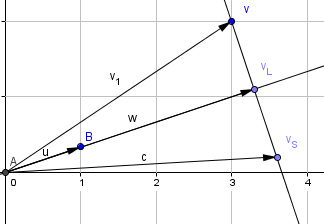
\includegraphics[scale=0.75]{graph_ans_3}

\section*{2.}
\subsection*{a)}
{\bf Normal form: }
$x+y-3=0$

\subsection*{b)}
{\bf Slope-intercept form: }
$y=-x+3$

\subsection*{c)}
{\bf Parameterform: }
$\left\{
\begin{array}{l l}
    x=1-3k\\
    y=2+3k
\end{array}\right.$

\section*{3.}
$A=(1,5)$\\
$s \equiv 2x+y+2=0$ $\Leftrightarrow$ $y=-2x-2$

\noindent
Parallella linjer $\Rightarrow$ $k_{r} = k_{s} = \frac{-2}{1}$\\
Sätt in $x$ och $y$ från punkt $A$ $\Rightarrow$ $y-5 = -2(x-1)$ $\Rightarrow$ 
$2x+y-7=0$\\

\section*{4}
Normalen till planet ges av $\overrightarrow{n}=\overrightarrow{AB} \times 
\overrightarrow{AC} = (20,16,-6)$\\
Vi kan sedan använda punkten $A$ och vektorn $\overrightarrow{n_{2}}=
(10,8,-3)$ som är parallell med $\overrightarrow{n}$.\\
$A(x-x_{1})+B(y-y_{1})+C(z-z_{1})=0 \Rightarrow \\
10(x-1)+8(y-1)-3(z+2)=0 \Rightarrow \\
10x+8y-3z-24=0$

\section*{5}
\subsection*{a)}
Pythagoras $\Rightarrow$ $$d = \sqrt{(9-3)^2+(7-2)^2} = \sqrt{61}$$

\subsection*{b)}
$$d = \frac{|Ax+By+C|}{\sqrt{A^2+B^2}} = 
      \frac{|(-2)(5)+(3)(6)+(4)|}{\sqrt{4+9}} = 
      3.328$$

\subsection*{c)}
$$d = \frac{|Ax+By+Cz+D|}{\sqrt{A^2+B^2+C^2}} = 
      \frac{|(2)(3)+(1)(1)+(1)(-2)+1|}{\sqrt{2^2+1^2+(-1)^2}} = 
      \frac{10}{\sqrt{6}}$$

\section*{6}
\subsection*{a)}
Addera cellvis.
$ 
    			\begin{bmatrix}
    			1-2 & 2+4 \\
    			5+6 & 9+1
    			\end{bmatrix}
    			=
    			\begin{bmatrix}
    			-1 & 6 \\
    			11  & 10
    			\end{bmatrix}
    			$
    			
\subsection*{b)}
Subtrahera cellvis.
$ 
    			\begin{bmatrix}
    			5-5 & -7-5 \\
    			4-(-2) & -1-8
    			\end{bmatrix}
    			=
    			\begin{bmatrix}
    			0 & -12 \\
    			6  & -9
    			\end{bmatrix}
    			$
    			
\subsection*{c)}
Tänk rad gånger kolumn.
$ 
    			\begin{bmatrix}
    			2*5+5*7  \\
    			2*2+3*7
    			\end{bmatrix}
    			=
    			\begin{bmatrix}
    			45  \\
    			25
    			\end{bmatrix}
    			$

\subsection*{d)}

$ 
    			\begin{bmatrix}
    			2*5+5*7 & 5*8+5*1  \\
    			2*2+3*7 & 2*8+3*1
    			\end{bmatrix}
    			=
    			\begin{bmatrix}
    			45 & 45\\
    			25 & 19
    			\end{bmatrix}
    			$

\subsection*{e)}
Här byter vi plats på raderna och kolumnerna.
				$ 
    			\begin{bmatrix}
    			5 & 4 \\
    			7 & -6 \\
    			9 & 9 
    			\end{bmatrix}
    			$
    			
    			
\section*{7}
\subsection*{a)}
				$ 
    			\begin{vmatrix}
   		 		7  & 4 \\
  		  		1  & 2
		    	\end{vmatrix}
		    	=
		    	7*2 - 1*4
		    	= 10
  			  	$
\subsection*{a)}
$Det(A) = 0 \implies \vec{u}$ och $\vec{v}$ är linjärt oberoende. Vilket betyder att vinkeln är skild från 0 och 180.

\section*{7}
\subsection*{a) }
	$ 
    			\begin{bmatrix}
    			7  & 2 \\
    			3  & 5
    			\end{bmatrix}
    			\cdot
    			\begin{bmatrix}
    			1 & 0  \\
    			0 & 1
    			\end{bmatrix}
    			=
    			\begin{bmatrix}
    			7  & 2 \\
    			3  & 5
    			\end{bmatrix}
    			$
    			
\subsection*{b) }
				$
				\begin{bmatrix}
    			7  & 2 \\
    			3  & 5
    			\end{bmatrix}
				^{-1}
				=
				\frac{1}{7*5-2*3}
				\begin{bmatrix}
    			5  & -2 \\
    			-3  & 7
    			\end{bmatrix}
				$
\subsection*{c) }
$				A A^{-1} = I =
				\begin{bmatrix}
    			1  & 0 \\
    			0  & 1
    			\end{bmatrix}
    			$ 
\subsection*{d) }
				$
				\begin{bmatrix}
    			a  & b \\
    			c  & d
    			\end{bmatrix}  
    			\cdot
    			\frac{1}{det(A)}
    			\begin{bmatrix}
    			d  & -b \\
    			-c & a
    			\end{bmatrix}
    			=
    			\frac{1}{det(A)}
    			\begin{bmatrix}
    			ad - bc  & -ab + ab \\
    			cd - cd  & -bc + ad
    			\end{bmatrix} 
    			=
    			\frac{1}{ad-bc}
    			\begin{bmatrix}
    			ad - bc  & -ab + ab \\
    			cd - cd  & -bc + ad
    			\end{bmatrix} 
    			=
    			\begin{bmatrix}
    			1 & 0 \\
    			0 & 1
    			\end{bmatrix} 
    			$
\end{document}
